\documentclass[12pt,a4paper]{article}
\usepackage[utf8]{inputenc}
\usepackage{graphicx}
\usepackage[none]{hyphenat}
\usepackage{hyperref}
\usepackage{xcolor}

\setlength{\fboxrule}{2pt}

\begin{document}
	\begin{titlepage}
		
		\begin{center}
			
\includegraphics[width=0.5\textwidth]{QUT.jpg}\\
			[0.03\textheight]  
			\Large\textbf{Bachelor of IT (Computer Science)}\\
			\Large\textbf{Assignment 2 - Client-Side React Application}\\
			\large\textbf{CAB230 - Web Computing}\\
			[0.02\textheight]
			\large\textsl{Dane Madsen}\\
			\large\textsl{n10983864@qut.edu.au}
		\end{center}
		
	\end{titlepage}
	\tableofcontents
	\newpage
	
	\section{Introduction}
		\subsection{Purpose and Description}
			The purpose of this react application is to collate and display information regarding movies, 
			and cast members to the user in a responsive and accessible manner. The application should 
			allow the user to search for movies by year or title and display the results in a list. 
			When a movie is selected, the application should display all the details of the movie, 
			including the year the movie was made, the plot of the movie and all the cast members 
			involved with the movie. The application should also allow the user to visit individual 
			pages of cast members where the user can view that cast members details, including their 
			birth year, death year and all the movies they have been involved with.\\
			\\
			It achieve this goal and to provide the user with the best experience I can, i have used a 
			number of advanced react features, including the use of react router, ag-grid and 
			react-responsive-carousel. The use of these features has allowed me to create a 
			professional looking application that is both easy to use and responsive for the user.\\

			\begin{center}
				\fbox{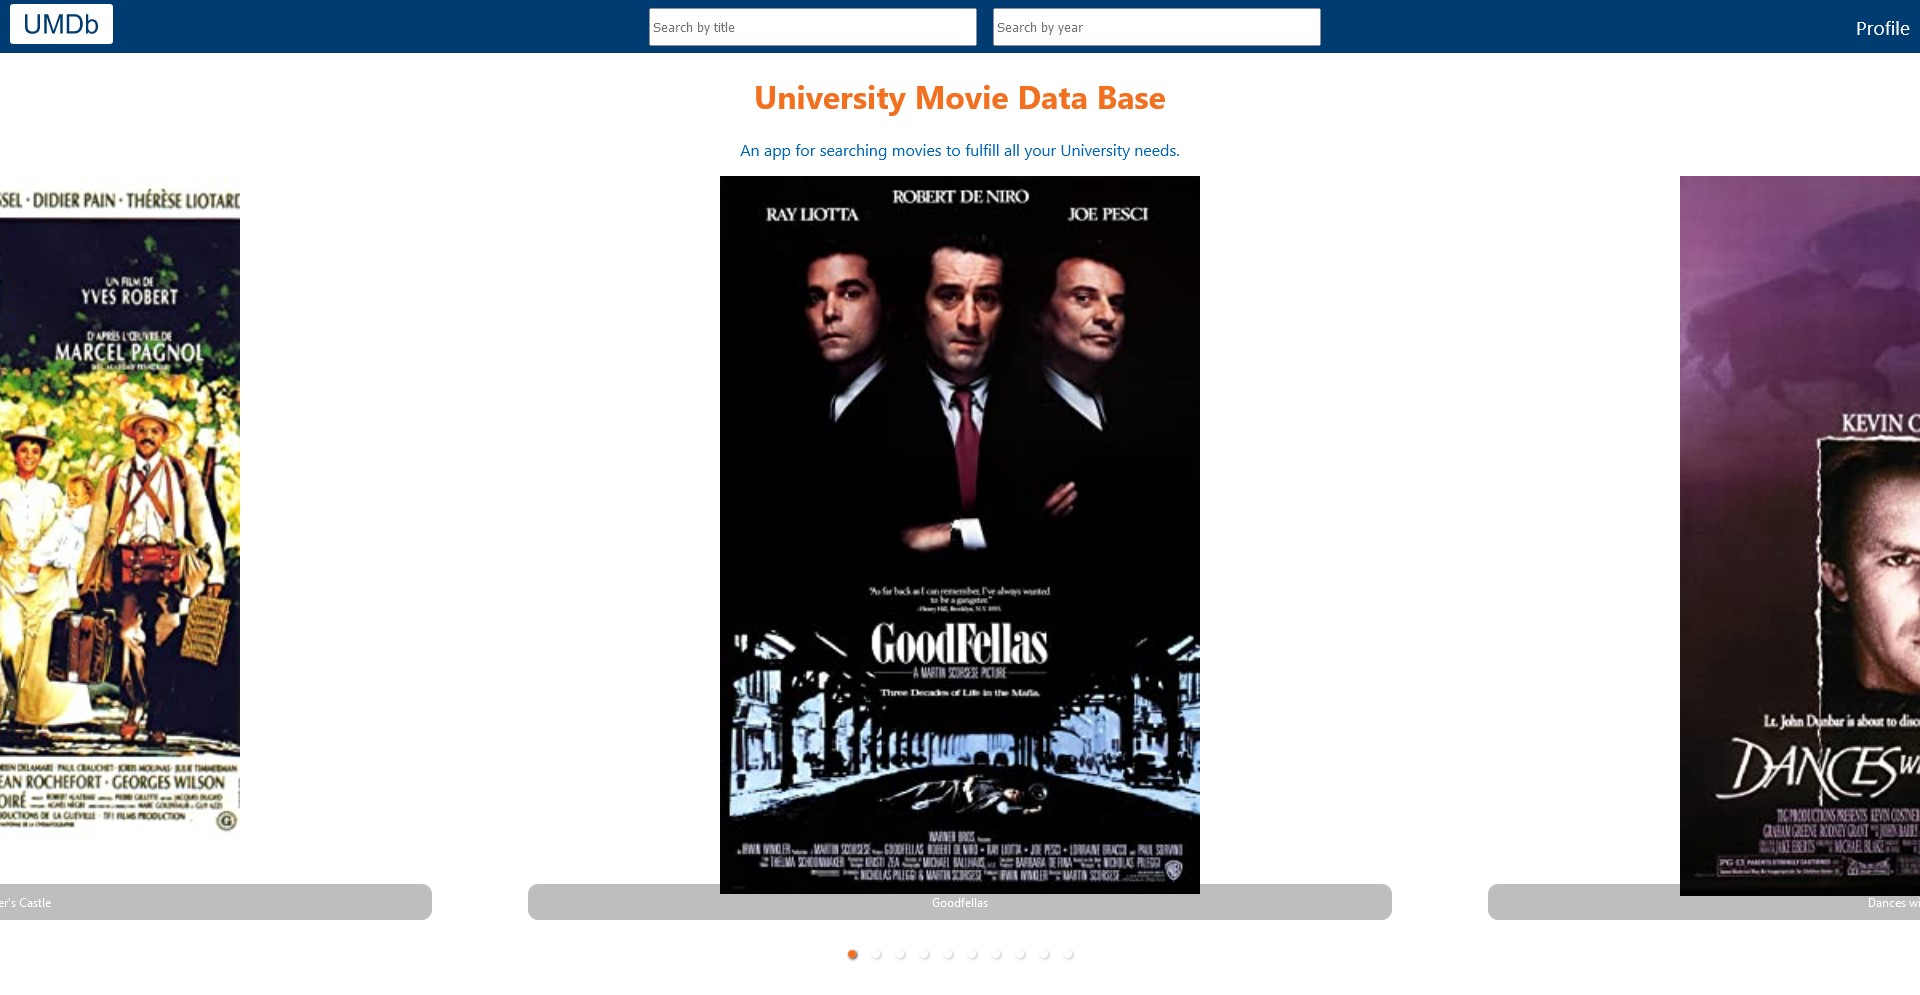
\includegraphics[width=\textwidth]{Figure1.jpg}}
				\fbox{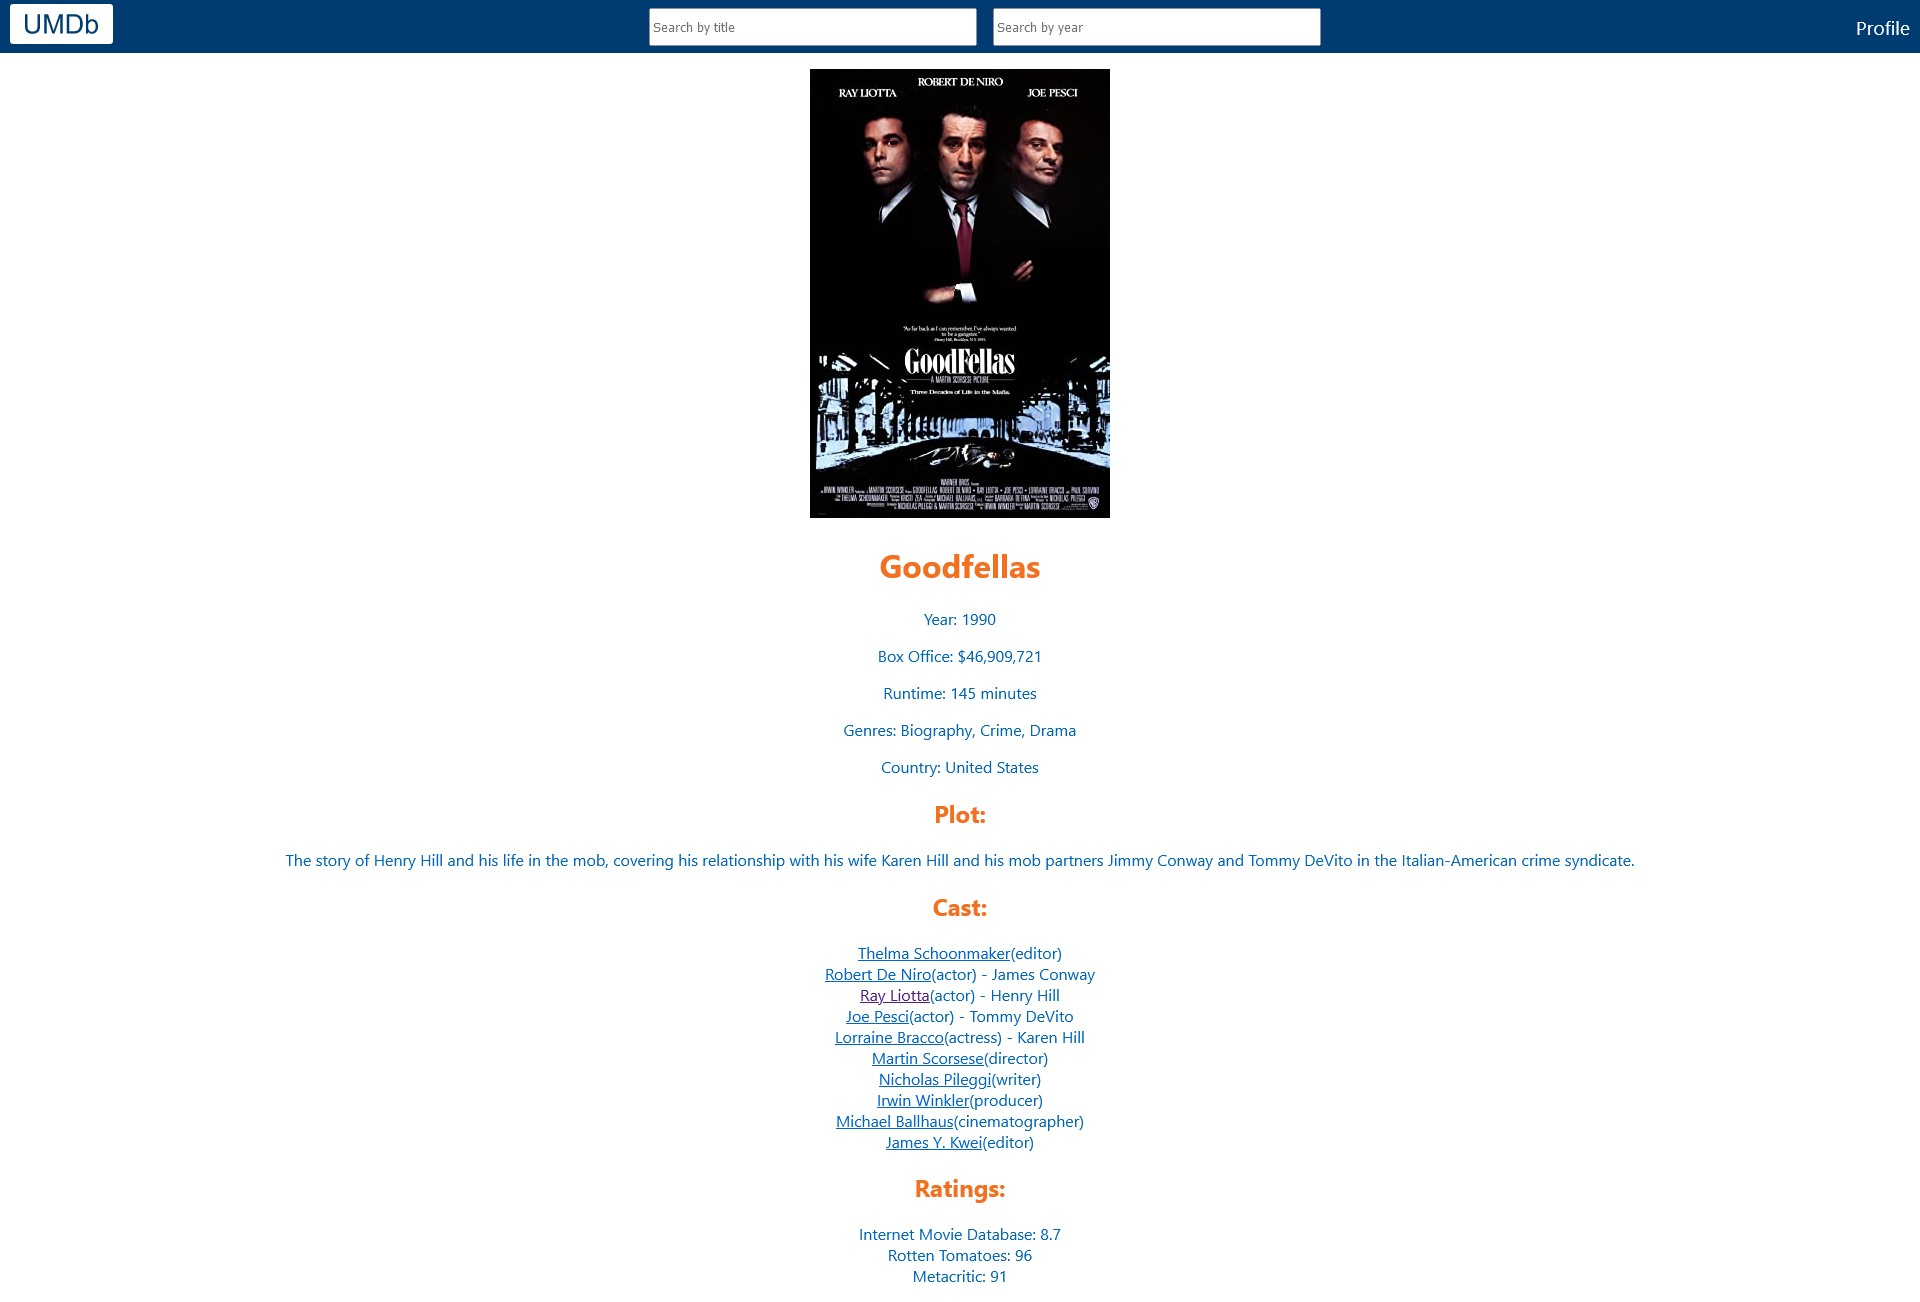
\includegraphics[width=\textwidth]{Figure2.jpg}}
			\end{center}
		
		\subsection{Completeness and Limitations}
			This implementation covers all the requirements of the assignment specification. 
			Navigation is handled using react router, controlled forms are used for all user input, and 
			every 10 minutes the refresh token is used to get a new access token. In addition to this, 
			the application uses ag-grid to display the search results and react-responsive-carousel 
			to display the highest scoring movies of all time on the home (landing) page.\\

	\section{Use of End Points}



\end{document}